\documentclass[convert={density=1024}]{standalone}
\usepackage{amsmath, amsthm, amsfonts}
\usepackage{tikz-cd, kotex}
\usepackage{../../preamble/quiver}

\begin{document}



\end{document}
%% Extend_by_linearity (Matrix-1.png)
\begin{tikzcd}
	{\mathcal{B}} & V \\
	& W
	\arrow["g"', from=1-1, to=2-2]
	\arrow["\iota", hook, from=1-1, to=1-2]
	\arrow["G", dashed, from=1-2, to=2-2]
\end{tikzcd}

%% Block_matrix (Matrix-2.png)
\newcommand{\bigzero}{\mbox{\normalfont\Large\bfseries 0}}
\newcommand{\rvline}{\hspace*{-\arraycolsep}\vline\hspace*{-\arraycolsep}}
$\displaystyle\begin{pmatrix}
  \bigzero
  & \rvline & \begin{matrix}1\\3\end{matrix} \\
\hline
  \begin{matrix} 2&4\end{matrix}& \rvline & 0
\end{pmatrix}$

%% Fundamental_theorem_of_linear_algebra (Fundamental_theorem_of_linear_algebra-1.png)
\begin{tikzcd}
\color{gray}v\ar[rrr, |->, gray]\dar[ddd, |->, gray]&[-20pt]&&[-30pt]\color{gray}L(v)\dar[ddd, |->, gray]\\[-15pt]
&V\rar["L"]\dar[-, double]&W\dar[-, double]\\
&F^n\rar["{[L]_\mathcal{C}^\mathcal{B}}" below]&F^m\\[-15pt]
\color{gray}{[v]_\mathcal{B}}\ar[rrr, |->, gray]&&&\color{gray}\substack{[L(v)]_\mathcal{C}\\[2pt]={[L]_\mathcal{C}^\mathcal{B}[v]_{\mathcal{B}}}}
\end{tikzcd}

%% Dual_map (Dual_space-1.png)
\begin{tikzcd}
	V & W \\
	& F
	\arrow["L", from=1-1, to=1-2]
	\arrow[""{name=0, anchor=center, inner sep=0}, "f", from=1-2, to=2-2]
	\arrow[""{name=1, anchor=center, inner sep=0}, "{f\circ L}"', dashed, from=1-1, to=2-2]
	\arrow[curve={height=3pt}, shorten <=3pt, shorten >=3pt, Rightarrow, from=0, to=1, "L^\ast" {font=\tiny, above=2pt}, pos=.3]
\end{tikzcd}

%% Parellelpiped (Determinant-1.png)
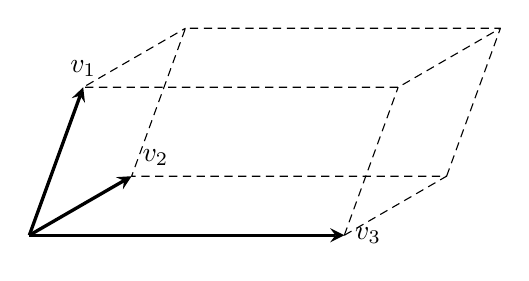
\begin{tikzpicture}
	\begin{scope}[x={(4cm,0cm)},y={({cos(30)*1.5cm},{sin(30)*1.5cm})},z={({cos(70)*2cm},{sin(70)*2cm})},line join=round]
		\draw[densely dashed] (1,0,0) -- (1,1,0) -- (0,1,0) -- (0,1,1) -- (1,1,1) -- (1,0,1) -- (0,0,1) -- (0,1,1);
		\draw[densely dashed] (1,0,0) -- (1,0,1);
		\draw[densely dashed] (1,1,0) -- (1,1,1);
		\draw[very thick, -{stealth}, black] (0,0,0)--(0,0,1) node[above]{$v_1$};
		\draw[very thick, -{stealth}, black] (0,0,0)--(0,1,0) node[above right]{$v_2$};
		\draw[very thick, -{stealth}, black] (0,0,0)--(1,0,0) node[right]{$v_3$};
	\end{scope}
\end{tikzpicture}

%% Square (Determinant-2.png)
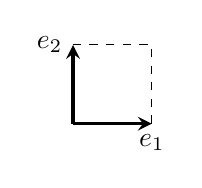
\begin{tikzpicture}
\draw[very thick, -{stealth}] (0,0)--(0,1) node[left]{$e_2$};
\draw[very thick, -{stealth}] (0,0)--(1,0) node[below]{$e_1$};
\draw[dashed] (1,0)--(1,1)--(0,1);
\end{tikzpicture}

%% Transformation (Determinant-3.png)
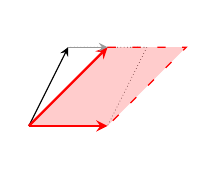
\begin{tikzpicture}
\draw[ -{stealth}] (0,0)--(0.5,1);
\draw[very thin,densely dotted] (0,0)--(1,0)--(1.5,1)--(0.5,1)--cycle;
\draw[thick, red, -{stealth}] (0,0)--(1,1) node[above]{};
\draw[thick, red, -{stealth}] (0,0)--(1,0) node[below]{};
\draw[red, loosely dashed] (1,1)--(2,1)--(1,0);
\fill[red, opacity=.2] (0,0)--(1,0)--(2,1)--(1,1)--cycle;
\draw[thin, black!40, -{stealth}] (0.5,1)--(1,1);
\end{tikzpicture}
\hspace{10pt}
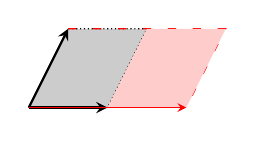
\begin{tikzpicture}
\filldraw[densely dotted, fill=black!20] (0,0)--(1,0)--(1.5,1)--(.5,1)--cycle;
\draw[thick, -{stealth}] (0,0)--(1,0);
\draw[thick, -{stealth}] (0,0)--(.5,1);
\draw[loosely dashed, red] (.5,1)--(2.5,1)--(2,0);
\fill[red!20] (1,0)--(2,0)--(2.5,1)--(1.5,1)--cycle;
\draw[red, -{stealth}] (0,0)--(2,0) node[below]{};
\end{tikzpicture}

%% Multilinearity (Determinant-4.png)
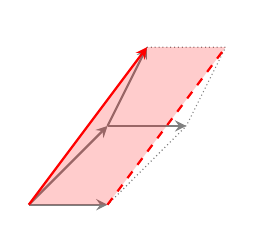
\begin{tikzpicture}
	\draw[thick, gray, -{stealth}] (0,0)--(1,0) node[below]{};
	\draw[thick, gray, -{stealth}] (0,0)--(1,1);
	\draw[thick, gray, -{stealth}] (1,1)--(1.5,2) node[above]{};
	\draw[gray, densely dotted] (1,1)--(2,1)--(1,0);
	\draw[gray, densely dotted] (1.5,2)--(2.5,2)--(2,1);
	\draw[gray, thick, -{stealth}] (1,1)--(2,1);
	\draw[thick, red, -{stealth}] (0,0)--(1.5,2);
	\draw[thick, dashed, red] (1,0)--(2.5,2);
	\fill[red, opacity=.2] (0,0)--(1,0)--(2.5,2)--(1.5,2)--cycle;
\end{tikzpicture}

%% Change-of-basis matrix (Change_of_basis-1.png)
\begin{tikzcd}
	V\rar["\operatorname{id}_V"]\dar&V\dar\\
	F^n\rar["{[\operatorname{id}_V]^\mathcal{B}_{\mathcal{B}'}}"]
\end{tikzcd}

%% B-identification (Bilinear_form-1.png)
\begin{tikzcd}
	{W^\ast} & {V^\ast} \\
	W & V
	\arrow["{L^\ast}", from=1-1, to=1-2]
	\arrow["{\varphi_W}"', from=1-1, to=2-1]
	\arrow["{\varphi_V}", from=1-2, to=2-2]
	\arrow["{L'}"', from=2-1, to=2-2]
\end{tikzcd}


